
\chapter{配对实验}
 \label{chapter::mpe}
 
配对实验（Matched-Pairs Experiment, MPE）是随机化实验（SRE）的极端形式：在每个分层内仅有一个处理组单位和一个对照组单位。此时这些分层也被称为“配对”。虽然这种实验形式属于第\ref{chapter::stratification-poststratification}章所述SRE的特殊情况，但它有自己独立的估计与推断方法。此外，它还具有许多新特性，且与第\ref{chapter::matching-obs}章将要讨论的观测研究中的“匹配”策略密切相关。因此我们在此单独设章探讨MPE。 





\section{实验设计及潜在结果}
 
考虑一个有$2n$个单位的实验。若存在可用于预测结果的协变量，则可依据协变量的相似性来配对单位。若协变量为标量，可先对单位按该值排序，再将相邻单位配对。若存在多个协变量，则可计算单位间的两两距离并据此配对。此时配对过程可采用贪婪算法或最优非二分匹配算法实现。贪婪算法会先配对距离最小的两个单位，将其从候选池移除，再对剩余单位重复此过程。最优非二分匹配算法则能将$2n$个单位划分为$n$个二元组，使得每组内距离之和最小。关于MPE计算层面的更多细节可参见\citet{greevy2004optimal}。本章假设配对已通过协变量完成，后续将讨论由此产生的设计与推断问题。 


 用$(i,j)$表示第$i$对中的第$j$个单位，其中$i=1,\ldots, n$、$j=1,2$。单位$(i, j)$在处理与对照下的潜在结果分别为$Y_{ij}(1)$和$Y_{ij}(0)$。每一对内随机选一人接受处理，另一人作为对照。令
$$
Z_i = \begin{cases}
   1,& \text{if the first unit receives the treatment}, \\
   0, & \text{if the second unit receives the treatment}. 
\end{cases}  
$$
据此，可通过处理分配机制正式定义配对实验（MPE）。 


\begin{definition}
[MPE]
满足以下条件：  
\begin{eqnarray}
 (Z_i)_{i=1}^n \iidsim \text{Bernoulli}(1/2).
 \label{eq::mp-treatment}
\end{eqnarray} 
\end{definition}

 
 
第$i$对的观测结果为
$$
Y_{i1} = Z_i Y_{i1}(1) + (1-Z_i) Y_{i1}(0)
= \begin{cases}
   Y_{i1}(1),& \text{if } Z_i = 1; \\
   Y_{i1}(0), & \text{if } Z_i = 0; 
\end{cases}
$$
和
$$
Y_{i2} = Z_i Y_{i2}(0) + (1-Z_i) Y_{i2}(1)
= \begin{cases}
   Y_{i2}(0),& \text{if } Z_i = 1; \\
   Y_{i2}(1), & \text{if } Z_i = 0 . 
\end{cases} 
$$
因此，观测数据为$( Z_i, Y_{i1} , Y_{i2} )_{i=1}^n$。  
 
 
\section{FRT}
 
 与前面的讨论类似，总可以用 FRT 检验尖锐零假设
$$
\HF: Y_{ij}(1) = Y_{ij}(0)  \text{ for all }  i=1,\ldots  n  \text{ and } j=1,2. 
$$
实施 FRT 时，需要根据\eqref{eq::mp-treatment}模拟$(Z_1, \ldots, Z_n)$的分布。下面介绍几种基于处理与对照结果对内差的常用统计量：
\begin{eqnarray*}
\hat{\tau}_i &=& \text{outcome under treatment} - \text{outcome under control} \text{ (within pair } i) \\
&=&  (2Z_i - 1) (Y_{i1}  - Y_{i2})\\
&=& S_i (Y_{i1}  - Y_{i2})  , 
\end{eqnarray*}
其中$S_i = 2Z_i - 1$是独立同分布的随机符号，均值为$0$，方差为$1$，$i=1,\ldots, n$。由于$\hat{\tau}_i $为零的配对不影响随机化分布，讨论 FRT 时将它们删除。 
 
\begin{example} 
[配对$t$统计量]\label{eg::paired-t-statistic}
对内差的平均值为
$$
\hat{\tau} = n^{-1}  \sumn \hat{\tau}_i .
$$
在$\HF$下，
$$
E(\hat{\tau} ) = 0
$$
且
$$
\var(  \hat{\tau}   ) 
= n^{-2} \sumn \var(  \hat{\tau}_i ) 
= n^{-2} \sumn \var(S_i) (Y_{i1}  - Y_{i2})^2 =  n^{-2} \sumn  \hat{\tau}_i^2 . 
$$
由独立随机变量和的中心极限定理，得到正态近似
$$
\frac{  \hat{\tau}  }{ \sqrt{  n^{-2} \sumn  \hat{\tau}_i^2 } } \rightarrow \N01 
$$
这里为依分布收敛，可据此构造渐近检验。许多标准教材建议在配对实验中使用如下配对$t$统计量：
$$
t_\text{pair} = \frac{  \hat{\tau}  }{ \sqrt{  \{ n(n-1) \}^{-1} \sumn  (\hat{\tau}_i - \hat{\tau} ) ^2 } },
$$
在$\HF$下，$n$较大、$\hat{\tau} $较小时，它与$\hat{\tau}$对应的标准化统计量几乎相同。 
\end{example} 

经典统计学在另一框架下论证$t_\text{pair}$的使用。若$\hat{\tau}_i \iidsim \textsc{N}(0, \sigma^2)$，可证明$t_\text{pair} \sim t(n-1)$，即$t_\text{pair} $精确服从自由度为$n-1$的$t$分布；$n$较大时，这接近$\N01$。在\ri{R}中，用\ri{t.test}函数并指定\ri{paired=TRUE}即可实施该检验。$n$较大时，这些方法结果相近。例\ref{eg::paired-t-statistic}无需假定数据正态，就为经典配对$t$检验提供了另一种依据。 

 
 
 

 
 
  \begin{example}
 [威尔科克森符号秩统计量]\label{eg::mpe-sign-rank}
根据$( | \hat{\tau}_1| , \ldots, | \hat{\tau}_n| )$的秩$(R_1, \ldots, R_n)$，定义统计量
$$
W = \sumn  I( \hat{\tau}_i > 0 ) R_i. 
$$
%Under $\HF$, we can drop the pairs with $ \hat{\tau}_i = 0$ since those pairs do not contribute to the randomization distribution of $W$. Ignoring those pairs with $ \hat{\tau}_i = 0$, we 
在$\HF$下，各$| \hat{\tau}_i|$固定，因而各$R_i$也固定，故
$$
E(W) = \frac{1}{2} \sumn R_i = \frac{1}{2} \sumn i = \frac{n(n+1)}{4}
$$
以及
$$
\var(W) = \frac{1}{4} \sumn R_i^2 = \frac{1}{4} \sumn i^2 = \frac{n(n+1)(2n+1)}{24}. 
$$
独立随机变量和的中心极限定理给出正态近似
$$
\frac{W - n(n+1)/4}{ \sqrt{n(n+1)(2n+1) / 24    } } \rightarrow \N01
$$
这里为依分布收敛，可据此构造渐近检验。\ri{R}中的\ri{wilcox.test}函数指定\ri{paired=TRUE}时，可以实施精确检验和渐近检验。 
 \end{example}
 
 
 
 
   \begin{example}
 [柯尔莫哥洛夫-斯米尔诺夫型统计量]\label{eg::mpe-ksstatistics}
在$\HF$下，绝对值$( | \hat{\tau}_1| , \ldots, | \hat{\tau}_n| )$固定，但符号随机，因此$   (  \hat{\tau}_1 , \ldots,  \hat{\tau}_n  )$与$ -   (  \hat{\tau}_1 , \ldots,  \hat{\tau}_n  )$应具有相同分布。令
$$
\hat{F}(t)  = n^{-1} \sumn I( \hat{\tau}_i  \leq t  )
$$
为$  (  \hat{\tau}_1 , \ldots,  \hat{\tau}_n  )$的经验分布，
$$
1 - \hat{F}(-t-)  =    n^{-1} \sumn I( -  \hat{\tau}_i  \leq t  )
$$
为$ -   (  \hat{\tau}_1 , \ldots,  \hat{\tau}_n  )$的经验分布，其中$\hat{F}(-t-)$表示函数$\hat{F}(\cdot)$在$-t$处的左极限。相应的 Kolmogorov--Smirnov 型统计量为
$$
D = \max_t |  \hat{F}(t)  +  \hat{F}(-t-)  - 1  |.
$$
\citet{butler1969test}提出了这一统计量，并推导了其精确和渐近分布。标准软件包尚未实现这一检验，但仍可通过 FRT 模拟精确分布并计算$p$值。\footnote{\citet{butler1969test}最初在稍有不同的框架下提出该统计量。若从分布$F(y)$独立同分布抽取$    (  \hat{\tau}_1 , \ldots,  \hat{\tau}_n  )$，且它们关于$0$对称，则
$$
F(t) = \pr( \hat{\tau}_i \leq t ) =  \pr( -  \hat{\tau}_i \leq t )  = 1 - \pr( \hat{\tau}_i <- t) = 1 - F(-t-).
$$
因此，$\hat{F}(t)  +  \hat{F}(-t-)  - 1 $衡量对称性零假设的偏离，这正是例\ref{eg::mpe-ksstatistics}中$D$的构造动机。另一种朴素做法是像例\ref{eg::ks-CRE}一样，直接比较处理组与对照组结果的经验分布，但这实际上破坏了配对结构。虽然它仍可用于配对实验的 FRT，却未体现实验的配对设计。}
 \end{example}
 
 
 
 
 
  \begin{example}
 [符号统计量]\label{eg::mpe-sign}
 符号统计量仅使用对内差的符号：
$$
 \Delta = \sumn I( \hat{\tau}_i > 0 ).
 $$
% Again the pairs with $\hat{\tau}_i = 0$ do not contribute to the randomization distribution of $ \Delta $, so we drop them without loss of generality. 
 在$\HF$下，
$$
 I( \hat{\tau}_i > 0 ) \iidsim \textup{Bernoulli}(1/2)
 $$
因而
$$
  \Delta \sim \textup{Binomial}(n, 1/2).
 $$
据此得到精确二项检验，可在\ri{R}中使用\ri{binom.test}函数并指定\ri{p=1/2}。利用中心极限定理，也可根据二项分布的正态近似实施检验：
$$
\frac{  \Delta - n/2 }{  \sqrt{n/4} } \rightarrow \N01 
$$
这里为依分布收敛。 
 \end{example}
 
 
 
 \begin{example}
 [二元结果下的麦克尼马尔检验]\label{eg::mcnenar-test-binary}
 若结果为二元变量，可更紧凑地汇总配对实验数据。每对中，处理结果可为$1$或$0$，对照结果可为$1$或$0$，从而得到表\ref{tb::binarymatchedpairs}的二乘二表。 
 
\begin{table}
\centering
\caption{四类配对的频数统计}\label{tb::binarymatchedpairs}
\begin{tabular}{ccc}
\hline 
 & 对照结果 1 & 对照结果 0\\
 \hline 
处理结果 1 & $m_{11}$ & $m_{10}$ \\
处理结果 0 & $m_{01}$ & $m_{00}$ \\
\hline 
\end{tabular}
\end{table} 
 
在$\HF$下，结果一致的配对数$m_{11}$和$m_{00}$固定，$m_{10} + m_{01}$也固定。唯一的随机分量为$m_{10}$，其分布为
$$
m_{10} \sim \textup{Binomial}( m_{10} + m_{01}, 1/2  ).
$$
由此得到精确二项检验。\ri{R}中的\ri{mcnemar.test}函数则利用二项分布的正态近似实施渐近检验：
$$
\frac{   m_{10}  - (m_{10} + m_{01})/2  }{  \sqrt{  (m_{10} + m_{01}) / 4   } } 
= \frac{ m_{10}  -  m_{01}   }{  \sqrt{ m_{10} + m_{01}    }  }
\rightarrow \N01  
$$
这里为依分布收敛。精确 FRT 与渐近检验都不依赖$m_{11}$或$m_{00}$，只有结果不一致的配对数影响检验。 
 \end{example}
 
 
 
\section{内曼推断法}
 
第$i$对内的平均因果效应为
$$
 \tau_i = \frac{1}{2}  \left\{    Y_{i1}(1) + Y_{i2}(1) -     Y_{i1}(0)  - Y_{i2}(0)     \right\},
 $$
所有单位的平均因果效应为
$$
\tau = n^{-1} \sumn  \tau_i  = (2n)^{-1} \sumn \sum_{j=1}^2 \{  Y_{ij}(1) - Y_{ij}(0)   \} .
$$
直观可知，$\hat{\tau}_i $是$ \tau_i $的无偏估计，因此$\hat{\tau}  $是$\tau$的无偏估计。也可计算$\hat{\tau}  $的方差。由于配对实验只是分层随机实验的特例，具体公式留作习题\ref{para::variance-mp-design}。 


但不能照搬分层随机实验的方法估计配对实验中$\hat{\tau}  $的方差。每对只有一个处理单位和一个对照单位，对内结果的样本方差无法定义，数据也不足以估计第$i$对内$\hat{\tau}_i $的方差。  


能否估计配对实验中$\hat{\tau}$的方差？先暂时离开配对实验，考虑经典独立同分布抽样。若各$\hat{\tau}_i$独立同分布，均值为$\mu$、方差为$\sigma^2$，则$\hat{\tau} = n^{-1} \sumn \hat{\tau}_i$的方差为$\sigma^2 / n$。$\sigma^2$的无偏估计量是样本方差$(n-1)^{-1} \sumn ( \hat{\tau}_i -  \hat{\tau} )^2$，所以$\var( \hat{\tau}  )$的无偏估计量为
\begin{equation}\label{eq::mpe-variance-estimation}
\hat{V} = \{ n(n-1)  \}^{-1} \sumn ( \hat{\tau}_i -  \hat{\tau} )^2.
\end{equation}
这个讨论也能推广到独立但不同分布的情形，见第\ref{chapter::basic-prob-append}章习题\ref{hw::inid}。这看似偏离了统计假设完全不同的配对实验，但至少启发了方差估计量$\hat{V} $：用$\hat{\tau}_i $的对间变异估计$\hat{\tau}  $的方差。它虽在另一组假设下推导，却是否也适用于配对实验？下面的定理\ref{thm::varianceest-mp}给出肯定答案。
 
\begin{theorem}\label{thm::varianceest-mp}
在配对实验下，\eqref{eq::mpe-variance-estimation}定义的$\hat{V}$是$\hat{\tau}  $真实方差的保守估计：
$$
E(  \hat{V}) - \var(   \hat{\tau}  ) = \{ n(n-1)  \}^{-1} \sumn  (\tau_i - \tau)^2 \geq 0  .
$$
若各对的$\tau_i$相同，则$E(  \hat{V} )  = \var(\hat{\tau}) .$。
\end{theorem}


定理\ref{thm::varianceest-mp}表明，在配对实验下，$\hat{V} $一般是保守方差估计量；若各对的平均因果效应相同，它就是无偏的。这有些出人意料，因为$\hat{V} $依赖各$ \hat{\tau}_i $的对间变异，而$ \var(   \hat{\tau}  ) $依赖每个$ \hat{\tau}_i $的对内变异。下面的证明有助于理解这一结果。 
 
 


\begin{myproof}{定理}{\ref{thm::varianceest-mp}}
回忆基本代数恒等式：$\sumn (a_i - \bar a)^2 = \sumn a_i^2 - n \bar{a}^2$，此式类比随机变量$W$的方差公式$\var(W) = E(W^2) - (EW)^2$。应用此式于以下步骤：  
\begin{eqnarray*}
n(n-1) E( \hat{V} ) &=& E\left\{   \sumn (\hat{\tau}_i - \hat{\tau})^2 \right\}  \\
&=&  E\left (    \sumn \hat{\tau}_i^2 - n \hat{\tau}^2  \right)   \\
&=& \sumn \{  \var(\hat{\tau}_i) + \tau_i^2 \} - n \{  \var(\hat{\tau})  + \tau^2 \}\\
&=& \sumn  \var(\hat{\tau}_i)  - n \var(\hat{\tau}) + \sumn  \tau_i^2 - n  \tau^2 \\
&=& n^2 \var(\hat{\tau})  - n \var(\hat{\tau})  + \sumn (\tau_i - \tau)^2.
\end{eqnarray*}
故得  
$$
E( \hat{V} )  = \var(\hat{\tau})  + \{ n(n-1)  \}^{-1}   \sumn (\tau_i - \tau)^2 \geq  \var(\hat{\tau})  .
$$
\end{myproof}




与其他实验的讨论类似，Neyman 方法依赖大样本近似：当$n\rightarrow \infty$且满足一定正则条件时，
$$
\frac{  \hat\tau  -  \tau }{  \sqrt{\var( \hat\tau )} } \rightarrow \N01
$$
依分布收敛。由于方差被保守估计，Wald 型置信区间
$$
 \hat\tau   \pm     z_{1-\alpha/2}  \sqrt{ \hat{V} }
$$
覆盖$\tau$的概率渐近不低于$1-\alpha$。



如下命题表明，点估计量$\hat\tau$与方差估计量$\hat{V}$均可方便地通过 OLS 得到。 

\begin{proposition}\label{prop::mpe-variance}
将向量$(\hat{\tau}_1, \ldots, \hat{\tau}_n)\tran$只对截距作 OLS 回归，所得截距系数及其方差估计分别恰好等于$\hat\tau$与$\hat{V}$。
\end{proposition}

  命题\ref{prop::mpe-variance}的证明留作习题\ref{para::seols-matchedpairs}。 
  
  

\section{协变量调整}



虽然设计阶段已经按协变量配对，匹配仍可能不完全，即$(X_{i1}\neq X_{i2})$；有时还观测到配对时未使用的额外协变量。此时可进一步调整协变量，提高估计效率。设单位$(i, j)$的协变量为$X_{ij} $。与完全随机实验类似，配对实验中也有两类一般的协变量调整策略。 



\subsection{FRT}

 
先考虑配对实验中协变量调整后的 FRT。对应于定义\ref{def::pseudo-y-frt}，可以根据结果对协变量拟合模型后的残差构造统计量，因为在尖锐零假设下，这些残差是固定值。一种常用做法是将所有观测$Y_{ij}$对$X_{ij}$作 OLS 回归，得到残差$\hat \varepsilon_{ij}$，再将$\hat \varepsilon_{ij}$当作观测结果构造检验统计量。\citet{rosenbaum2002covariance}特别倡导在配对实验中采用这一方法。 


对应于定义\ref{def::model-out-frt}，也可直接使用模型拟合的某些系数作为检验统计量。下一小节将给出这种策略的一种统计量选择。 



\subsection{回归调整}


下面着重估计$\tau$。与结果一样，可计算协变量的对内差$\hat{\tau}_{X,i} $及其平均$\hat{\tau}_X $。可以证明
$$
 E(\hat{\tau}_{X,i}   ) = 0,\quad 
 E(\hat{\tau}_X ) = 0,
 $$
和
$$
\cov(\hat{\tau}_X   ) =n^{-2} \sumn \hat{\tau}_{X,i}   \hat{\tau}_{X,i}  \tran .
%= n^{-2} \sumn |  \hat{\tau}_{X,i}  |  |\hat{\tau}_{X,i}  | \tran  .
$$
在一次实际配对实验中，除非各$\hat{\tau}_{X,i}  $均为零，否则$\cov(\hat{\tau}_X   ) $不为零。若随机抽到的$(Z_1,\ldots, Z_n)$不理想，$\hat{\tau}_X $可能显著偏离零。与第\ref{sec::lin=adjustingforimbalance}节完全随机实验的讨论类似，调整协变量均值的不平衡，有望提高估计效率。 

类似于第\ref{sec::lin=adjustingforimbalance}节，考虑以$\gamma$为参数的一类估计量：
$$
\hat{\tau}(\gamma) = \hat{\tau} - \gamma\tran \hat{\tau}_X 
$$
对任意固定$\gamma$，其均值为$\tau$。希望选择$\gamma$使$\hat{\tau}(\gamma)$的方差最小。方差是$\gamma$的二次函数：
\begin{eqnarray*}
\var\{ \hat{\tau}(\gamma) \} &=&   \var(\hat{\tau} - \gamma\tran \hat{\tau}_X ) \\
&=&  \var(\hat{\tau}  ) + \gamma\tran \cov(\hat{\tau}_X   ) \gamma - 2\gamma\tran \cov( \hat{\tau}_X ,  \hat{\tau}  ),
\end{eqnarray*}
在
$$
\tilde{\gamma} = \cov(\hat{\tau}_X   )^{-1}  \cov( \hat{\tau}_X ,  \hat{\tau}  ).
$$
处达到最小。上文已得$\cov(\hat{\tau}_X   ) $的公式，也可写为
$$
\cov(\hat{\tau}_X   ) = n^{-2} \sumn |  \hat{\tau}_{X,i}  |  |\hat{\tau}_{X,i}  | \tran,
$$
其中$| \cdot | $表示向量逐分量取绝对值。因此，$\cov(\hat{\tau}_X   ) $是固定的，且可由观测数据得知。但$\cov( \hat{\tau}_X ,  \hat{\tau}  )$依赖未知潜在结果。幸运的是，仍可得到它的无偏估计量，见下面的定理\ref{thm::covariance-mp}。

\begin{theorem}\label{thm::covariance-mp}
$\cov( \hat{\tau}_X ,  \hat{\tau}  )$的无偏估计量为
$$
\hat{\theta} = \{n(n-1)  \}^{-1} \sumn ( \hat{\tau}_{X,i}  -  \hat{\tau}_{X} ) (   \hat{\tau}_i -  \hat{\tau}   ).
$$
\end{theorem}

定理\ref{thm::covariance-mp}的证明与定理\ref{thm::varianceest-mp}类似，留作习题\ref{para::covariance-est-proof}。 


因此，可用
\begin{eqnarray*}
\hat{\gamma} &=&  \left( n^{-2} \sumn \hat{\tau}_{X,i}   \hat{\tau}_{X,i}  \tran  \right)^{-1}
\left\{ \{n(n-1)  \}^{-1} \sumn (\hat{\tau}_{X,i}  -  \hat{\tau}_X )(   \hat{\tau}_i -  \hat{\tau}   ) \right\} \\
&\approx &  \left(  \sumn(  \hat{\tau}_{X,i}   - \hat{\tau}_X ) ( \hat{\tau}_{X,i}  -  \hat{\tau}_X  )\tran  \right)^{-1}
  \sumn (\hat{\tau}_{X,i}  -  \hat{\tau}_X ) (   \hat{\tau}_i -  \hat{\tau}   )  ,
\end{eqnarray*}
估计最优系数$\tilde{\gamma}$；它近似等于将各$\hat{\tau}_i $对$\hat{\tau}_{X,i} $作带截距 OLS 回归时$\hat{\tau}_{X,i}$的系数。最终估计量为
$$
\hat{\tau}_{\text{adj}} = 
\hat{\tau}( \hat{\gamma} ) = \hat{\tau} - \hat{\gamma} \tran \hat{\tau}_X  ,
$$
由 OLS 的性质，它近似等于将各$\hat{\tau}_i $对$\hat{\tau}_{X,i} $作带截距 OLS 回归得到的截距。


相应地，$\hat{\tau}_{\text{adj}} $的保守方差估计量为
\begin{eqnarray*}
\hat{V} _{\text{adj}} 
&=& 
\hat{V} + \hat \gamma\tran \cov(\hat{\tau}_X   ) \hat \gamma - 2 \hat \gamma\tran \hat \theta  \\
&=& \hat{V}  - \hat \theta \tran \cov(\hat{\tau}_X   ) ^{-1}    \hat \theta .
\end{eqnarray*}


一个微妙的技术问题是：$\hat\tau(\hat\gamma)$是否具有$\hat\tau(\tilde\gamma)$同样的最优性？在讨论\citet{lin2013}的估计量时已遇到类似问题。大样本下，可证明$\hat\tau(\hat\gamma) - \hat\tau(\tilde\gamma) =  - (\hat\gamma - \tilde\gamma)\tran \hat{\tau}_X $为更高阶小量，因为它是$\hat\gamma - \tilde\gamma$与$\hat{\tau}_X$两个“小”量的乘积。 


此外，\citet{fogarty2018regression}讨论了上述协变量调整过程的渐近等价回归形式，并严格证明了对应的中心极限定理。下面概括这一回归表述，略去正则条件。 


\begin{proposition}\label{prop::colin2018regression}
在配对实验中，将各$\hat{\tau}_i $组成的向量对$1$及各$\hat{\tau}_{X,i} $组成的矩阵作 OLS 回归，所得截距及其方差估计可方便地近似协变量调整估计量$\hat{\tau}_{\textup{adj}} $及对应的方差估计量$\hat{V} _{\textup{adj}}$。 
\end{proposition}


命题\ref{prop::colin2018regression}的证明留作习题\ref{para::seols-matchedpairs}。有意思的是，命题\ref{prop::mpe-variance}和\ref{prop::colin2018regression}都不需要对方差估计量作 EHW 修正，技术细节见\citet{fogarty2018regression}。由于将配对实验数据化为对内差，这里也无需对协变量中心化，与完全随机实验下\citet{lin2013}估计量的实现不同。

 


\section{实例演示}

\subsection{Darwin 比较异花授粉与自花授粉对玉米株高影响的数据}
\label{sec::frt-darwin-mpe}

这是\citet{Fisher:1935}中的经典例子，包含 15 对异花授粉或自花授粉的玉米，以株高为结果。\ri{R}的\ri{HistData}包提供原始数据，\ri{cross}与\ri{self}分别是异花授粉和自花授粉的株高，\ri{diff}表示二者之差。 

\begin{lstlisting}
> library("HistData")
> ZeaMays
   pair pot  cross   self   diff
1     1   1 23.500 17.375  6.125
2     2   1 12.000 20.375 -8.375
3     3   1 21.000 20.000  1.000
4     4   2 22.000 20.000  2.000
5     5   2 19.125 18.375  0.750
6     6   2 21.500 18.625  2.875
7     7   3 22.125 18.625  3.500
8     8   3 20.375 15.250  5.125
9     9   3 18.250 16.500  1.750
10   10   3 21.625 18.000  3.625
11   11   3 23.250 16.250  7.000
12   12   4 21.000 18.000  3.000
13   13   4 22.125 12.750  9.375
14   14   4 23.000 15.500  7.500
15   15   4 12.000 18.000 -6.000
\end{lstlisting}
 


该配对实验共有$2^{15} = 32768$种可能处理分配，用\ri{R}可以处理这一规模。下面的函数枚举所有处理分配：

\begin{lstlisting}
MP_enumerate = function(i, n.pairs) 
{
 if(i > 2^n.pairs)  print("i is too large.")
 a = 2^((n.pairs-1):0)
 b = 2*a
 2*sapply(i-1, 
          function(x) 
            as.integer((x %% b)>=a)) - 1
}
\end{lstlisting}



因此，枚举全部处理分配，计算相应的各$\hat{\tau}$及单侧精确$p$值。 

\begin{lstlisting}
> difference = ZeaMays$diff 
> n.pairs    = length(difference)
> abs.diff   = abs(difference)
> t.obs      = mean(difference)
> t.ran      = sapply(1:2^15, 
+                     function(x){ 
+                       sum(MP_enumerate(x, 15)*abs.diff) 
+                       })/n.pairs
> pvalue     = mean(t.ran>=t.obs)
> pvalue
[1] 0.02633667
\end{lstlisting}

图\ref{fig::frt-darwin-mpe}展示了$\HF$下$\hat{\tau}$的精确随机化分布。

\begin{figure}[th]
\centering
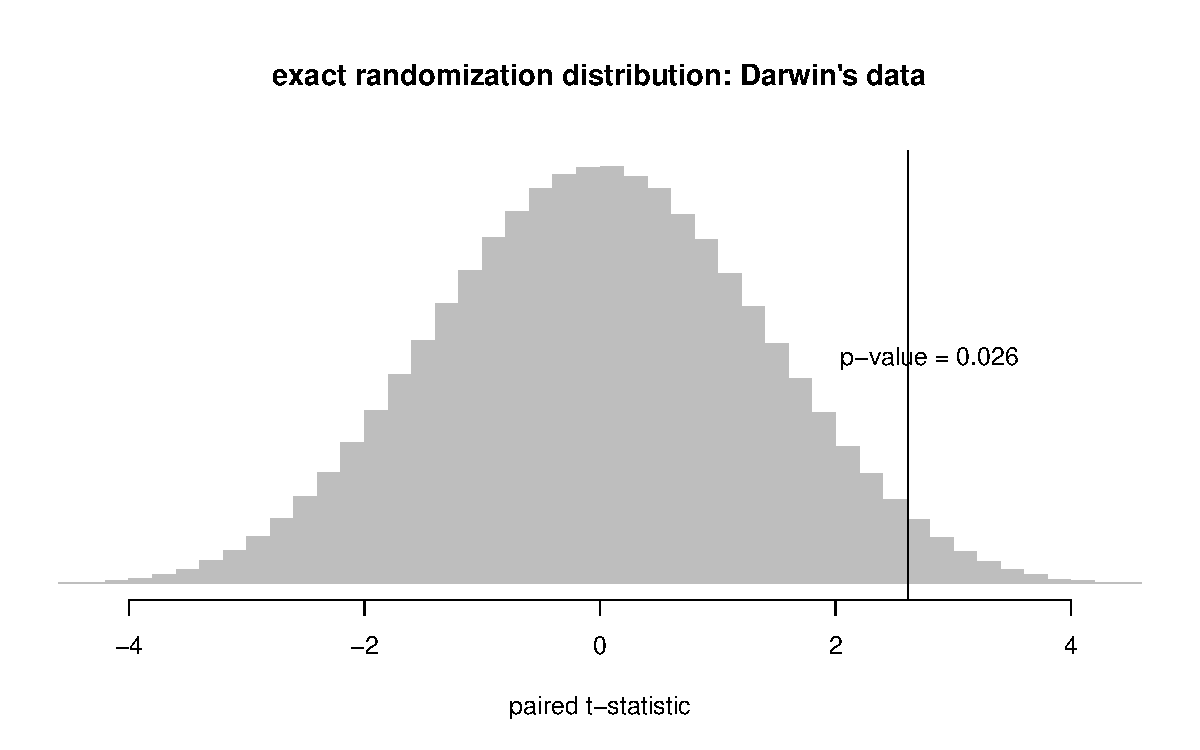
\includegraphics[width = \textwidth]{figures/frt_darwin.pdf}
\caption{利用 Darwin 数据得到的$\hat{\tau}$精确随机化分布}\label{fig::frt-darwin-mpe}
\end{figure}



\subsection{儿童电视教育实验数据}
\label{sec::neyman-television-mpe}



还重新分析了\citet{ball1973reading}中儿童电视工作坊实验的数据子集，\citet[][Chapter 10]{imbens2015causal}也分析过该数据。实验包含 8 对班级，每对随机选一个班，在正常阅读课时间观看{\it《电力公司》}节目。数据包含前测成绩（协变量）和后测成绩（结果）。下表汇总了对内协变量与结果及它们的差值：
\begin{lstlisting}
> dataxy = c(12.9, 12.0, 54.6, 60.6,
+            15.1, 12.3, 56.5, 55.5,
+            16.8, 17.2, 75.2, 84.8,
+            15.8, 18.9, 75.6, 101.9,
+            13.9, 15.3, 55.3, 70.6,
+            14.5, 16.6, 59.3, 78.4,
+            17.0, 16.0, 87.0, 84.2,
+            15.8, 20.1, 73.7, 108.6)
> dataxy = matrix(dataxy, 8, 4,  byrow = TRUE)           
> diffx = dataxy[, 2] - dataxy[, 1]
> diffy = dataxy[, 4] - dataxy[, 3]
> dataxy = cbind(dataxy, diffx, diffy)
> rownames(dataxy) = 1:8
> colnames(dataxy) = c("x.control", "x.treatment", 
+                      "y.control", "y.treatment",
+                      "diffx", "diffy")
> dataxy = as.data.frame(dataxy)
> dataxy
  x.control x.treatment y.control y.treatment diffx diffy
1      12.9        12.0      54.6        60.6  -0.9   6.0
2      15.1        12.3      56.5        55.5  -2.8  -1.0
3      16.8        17.2      75.2        84.8   0.4   9.6
4      15.8        18.9      75.6       101.9   3.1  26.3
5      13.9        15.3      55.3        70.6   1.4  15.3
6      14.5        16.6      59.3        78.4   2.1  19.1
7      17.0        16.0      87.0        84.2  -1.0  -2.8
8      15.8        20.1      73.7       108.6   4.3  34.9
\end{lstlisting}


下面的\ri{R}代码计算$\hat\tau$与$\hat V$。 
\begin{lstlisting}
> n      = dim(dataxy)[1]
> tauhat = mean(dataxy[, "diffy"])
> vhat   = var(dataxy[, "diffy"])/n
> tauhat
[1] 13.425
> sqrt(vhat)
[1] 4.636337
\end{lstlisting}
由命题\ref{prop::mpe-variance}和\ref{prop::colin2018regression}，可用 OLS 得到点估计与标准误。调整协变量后，有
\begin{lstlisting}
> unadj = summary(lm(diffy ~ 1, data = dataxy))$coef
> round(unadj, 3) 
            Estimate Std. Error t value Pr(>|t|)
(Intercept)   13.425      4.636   2.896    0.023
\end{lstlisting}
调整协变量后，有
\begin{lstlisting} 
> adj = summary(lm(diffy ~ diffx, data = dataxy))$coef
> round(adj, 3)
            Estimate Std. Error t value Pr(>|t|)
(Intercept)    8.994      1.410   6.381    0.001
diffx          5.371      0.599   8.964    0.000
\end{lstlisting}


这些结果要求$n$较大，只有认可大$n$近似，$p$值才有依据。但本例的$n=8$并不大，总共只有$2^8 = 256$种处理分配，所以最小可能$p$值是$1/256 = 0.0039$，远大于协变量调整估计量正态近似给出的$p$值。因此，更合理的做法是以学生化统计量——\ri{lm}函数给出的\ri{t value}——实施 FRT，计算精确$p$值。\footnote{其依据见第\ref{chapter::unification-fisher-neyman}章。}下面的\ri{R}代码计算基于两种$t$统计量的$p$值。 
\begin{lstlisting} 
> t.ran = sapply(1:2^8, function(x){ 
+   z.mpe = MP_enumerate(x, 8)
+   diffy.mpe = diffy*z.mpe
+   diffx.mpe = diffx*z.mpe
+   
+   c(summary(lm(diffy.mpe ~ 1))$coef[1, 3],
+     summary(lm(diffy.mpe ~ diffx.mpe))$coef[1, 3]) 
+ })
> p.unadj = mean(abs(t.ran[1, ]) >= abs(unadj[1, 3]))
> p.unadj
[1] 0.03125
> p.adj = mean(abs(t.ran[2, ]) >= abs(adj[1, 3]))
> p.adj
[1] 0.0078125
\end{lstlisting}


图\ref{fig::frt-television-mpe}给出了两个学生化统计量的精确分布及双侧$p$值。图中突出显示，检验统计量的随机化分布是离散的，至多只有 256 个取值。正态近似未必准确，尾部尤其如此，故应报告基于 FRT 的$p$值。 


\begin{figure}[th]
\centering
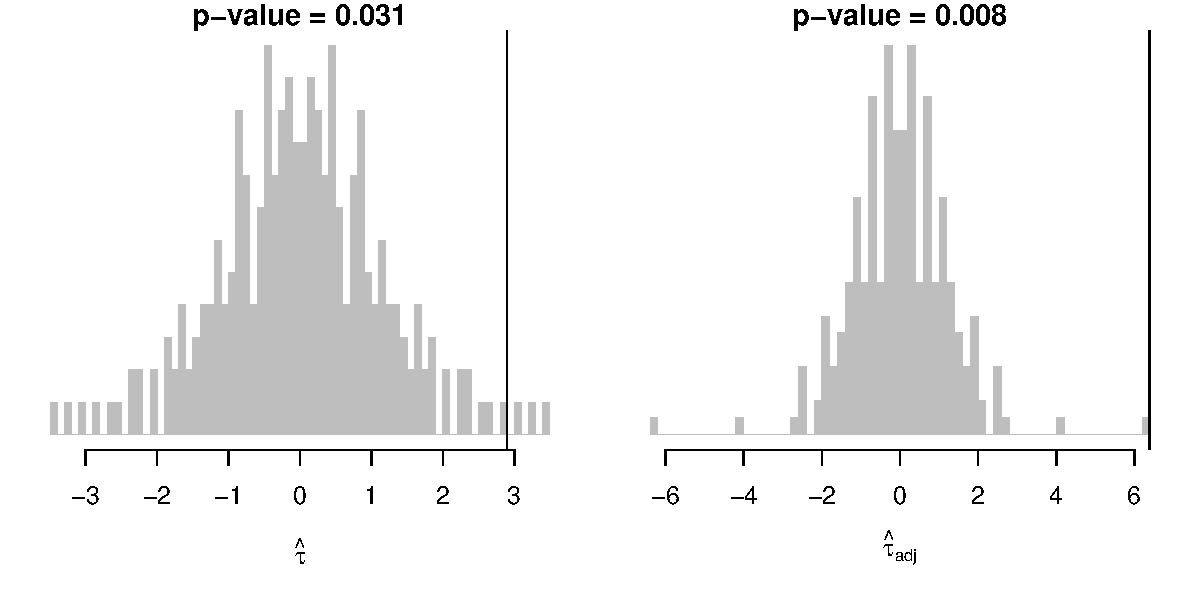
\includegraphics[width = \textwidth]{figures/frt_television.pdf}
\caption{第\ref{sec::neyman-television-mpe}节中学生化统计量的精确随机化分布}\label{fig::frt-television-mpe}
\end{figure}



\section{MPE与CRE的比较}
\label{sec::discussion}

\citet{imai2008variance}比较了配对实验与完全随机实验。直观上，若匹配良好且协变量能够预测结果，配对实验的估计更精确，但在设计阶段没有结果数据，难以判断这一条件是否满足。对于 FRT，若协变量能预测结果，配对实验通常比完全随机实验具有更高功效；\citet{greevy2004optimal}用基于 Wilcoxon 符号秩统计量的模拟说明了这一点。但有限样本下问题更微妙。考虑有$2n$个单位的实验，其中$n$个接受处理，$n$个作为对照。在$0.05$水平检验尖锐零假设时，配对实验至少需要$2\times 5=10$个单位，因为最小$p$值为$1/2^5 = 1/32 < 0.05$，但$1/2^4 = 1/16 > 0.05$；完全随机实验则至少需要$2\times 4 = 8$个单位，因为最小$p$值为$1/\binom{8}{4} = 1/70 < 0.05$，但$1/\binom{6}{3} = 1/20 = 0.05$。因此，只有$8$个单位时，配对实验不可能拒绝尖锐零假设，完全随机实验却有可能。即使协变量完美预测结果，按 FRT 衡量，配对实验也未必优于完全随机实验。 



\section{广义配对实验的推广}\label{sec::general-matched-experiment}

配对实验可直接推广为对照单位数可变的一般匹配实验。设有$n$个匹配集，编号为$i=1, \ldots, n$；第$i$个匹配集有$1+M_i$个单位，各$M_i$可以不同。实验总单位数为$N = n + \sum_{i=1}^n M_i$。用$ij$表示第$i$个匹配集中的第$j$个单位，其中$i=1,\ldots, n$、$j=1,\ldots, M_i+1$。单位$ij$的处理与对照潜在结果分别为$Y_{ij}(1)$和$Y_{ij}(0)$。 


在每个匹配集$i$中（$(i=1, \ldots, n)$），随机选且仅选一个单位接受处理，其余$M_i$个单位作为对照。这也是分层随机实验的特例：共有$n$层，各层大小为$1+M_i$，$(i=1, \ldots, n)$。令$Z_{ij}$为单位$ij$的处理指标，则观测结果为
$$
Y_{ij} = Z_{ij} Y_{ij}(1) + (1-Z_{ij}) Y_{ij}(0) . 
$$ 

匹配集$i$内的平均因果效应为
$$
\tau_i = (M_i + 1)^{-1} \sum_{j=1}^{1+M_i} \{ Y_{ij}(1)-Y_{ij}(0) \}. 
$$
由于一般匹配实验是分层随机实验，$\tau_i $的无偏估计量为
$$
\hat \tau_i = \sum_{j=1}^{M_i + 1} Z_{ij} Y_{ij} - M_i^{-1} \sum_{j=1}^{M_i+1} (1-Z_{ij}) Y_{ij}
$$
即匹配集$i$内的结果均值差。 

下面讨论一般匹配实验中的统计推断。 


\subsection{FRT}

同样，总可用 FRT 检验尖锐零假设
$$
\HF: Y_{ij}(1) = Y_{ij}(0)  \text{ for all }  i=1,\ldots, n; j=1,\ldots, M_i+1. 
$$
一般匹配实验是含许多小层的分层随机实验的特例，因此可使用例\ref{eg::hodgeslehmann}、\ref{eg::ks-stratified}、\ref{eg::mpe-sign-rank}、\ref{eg::mpe-ksstatistics}、\ref{eg::mpe-sign}的统计量，以及下面两小节的估计量及对应$t$统计量。 



\subsection{估计层内效应的平均值}


先考虑估计层内效应的平均值
$$
\tau = n^{-1} \sumn \tau_i .
$$
其无偏估计量为
$$
\hat\tau = n^{-1} \sumn \hat \tau_i . 
$$
有意思的是，定理\ref{thm::varianceest-mp}以及配对实验的其他结论仍适用于一般匹配实验。特别地，将各$\hat \tau_i $只对截距作 OLS 回归，就可得到$\tau$的点估计和方差估计。有协变量时，则将各$\hat \tau_i $对截距与各$\hat\tau_{X,i}$作 OLS 回归，其中
$$
\hat \tau_{X,i} = \sum_{j=1}^{M_i + 1} Z_{ij} X_{ij} - M_i^{-1} \sum_{j=1}^{M_i+1} (1-Z_{ij}) X_{ij}
$$
是匹配集$i$内相应的协变量均值差。 



\subsection{更一般的因果估计目标}


上面的$\tau$是各$\tau_i$的简单平均；各$M_i$不同时，它不等于实验中$N$个单位的平均因果效应。后者为
$$
\tau' = N^{-1} \sumn \sum_{j=1}^{1+M_i} \{ Y_{ij}(1)-Y_{ij}(0) \} = \sumn \frac{1+M_i}{N} \tau_i.
$$
为统一讨论，考虑加权因果效应
$$
\tau_w =  \sumn w_i \tau_i
$$
其中$\sumn w_i = 1$。它包括$w_i = n^{-1}$时的$\tau$，也包括对每个$i=1,\ldots, n$取$w_i = (1+M_i)/N $时的$\tau'$。容易得到无偏估计量
$$
\hat\tau_w =  \sumn w_i \hat\tau_i,
$$
及其方差
$$
\var(\hat\tau_w ) = \sumn w_i^2 \var (\hat\tau_i ). 
$$
但估计$\hat\tau_w $的方差相当棘手，因为各$\hat\tau_i$独立，却各自没有重复观测。这是\citet{hartley1969variance}和\citet{rao1970estimation}研究过的经典理论统计问题；\citet{fogarty2018mitigating}也讨论过，但未注意到这些早期工作。这里直接给出方差估计量，不详述构造动机：
$$
\hat{V}_w = \sumn c_i (\hat\tau_i -\hat\tau_w )  ^2
$$
其中
$$
c_i = \frac{    \frac{w_i^2}{1-2w_i}   }{   1 + \sumn  \frac{w_i^2}{1-2w_i} }.
$$
作为核查，配对实验中$M_i=1$且$w_i = n^{-1}$时，$c_i $简化为$ \{  n(n-1) \}^{-1}$。为简化讨论，假定对所有$i$均有$w_i < 1/2$，即没有任何匹配集占总权重的一半以上。下面的定理推广了定理\ref{thm::varianceest-mp}。  

\begin{theorem}
\label{thm::hadamdard-matched-experiment}
在各$M_i$可变的一般匹配实验中，若对所有$i$都有$w_i < 1/2$，则
$$
 E(\hat{V}_w ) - \var( \hat\tau_w  ) = \sumn c_i (\tau_i - \tau_w )^2 \geq \var( \hat\tau_w  )  \geq 0
 $$
各$\tau_i $相同时取等号。 
\end{theorem}

虽然$\hat{V}_w $的理论动机较复杂，直接验证定理\ref{thm::hadamdard-matched-experiment}却不太困难，证明留作习题\ref{para::variance-general-matched}。 
 



\section{作业习题}

\paragraph{MPE中$\hat{\tau}$的真实方差}
\label{para::variance-mp-design}

用潜在结果的有限总体方差表达$\var(\hat{\tau})$。 

\paragraph{协方差估计量的证明}\label{para::covariance-est-proof}
证明定理\ref{thm::covariance-mp}。

\paragraph{OLS方差估计方法}\label{para::seols-matchedpairs}
证明命题\ref{prop::mpe-variance}与\ref{prop::colin2018regression}。 


\paragraph{二元结果下的内曼推断}\label{para::binary-matchedpairs-neyman}


本题将例\ref{eg::mcnenar-test-binary}推广到 Neyman 推断。 

用表\ref{tb::binarymatchedpairs}中的计数表示$\hat\tau$与$\hat V$。 




\paragraph{最小样本量与FRT}
\label{prob::minimum-n-0.001}

推广第\ref{sec::discussion}节的讨论。考虑有$2n$个单位的实验，其中$n$个接受处理，$n$个作为对照，在$0.001$水平检验尖锐零假设。对于配对实验，要使最小$p$值不超过$0.001$，$n$至少应取多少？完全随机实验中相应的最小$n$是多少？
 

\paragraph{达尔文数据再分析}  
用威尔科克森统计量与内曼法重新分析该数据。

 
第\ref{sec::frt-darwin-mpe}节用统计量$\hat{\tau}$的 FRT 分析了 Darwin 数据。

改用 Wilcoxon 符号秩统计量的 FRT，重新分析该数据集。

采用 Neyman 推断重新分析该数据集，报告无偏点估计、保守方差估计及 95\% 置信区间。

\paragraph{电视实验数据再分析}  
对比不同检验法的结果差异。

第\ref{sec::neyman-television-mpe}节基于 Neyman 推断分析了这一数据集。

使用不同检验统计量的 FRT 重新分析该数据集。 

进行协变量调整，再用 FRT 重新分析该数据集。




\paragraph{重新分析\citet{angrist2009effects}的数据}\label{para::AL-mpe-neyman}

\citet{angrist2009effects}的原分析相当复杂。本题只关注原论文表 A1，并将学校视为实验单位。\citet{angrist2009effects}本质上对学校实施了配对实验。删除第 6 对及所有存在不依从的配对后，剩下 14 个完整配对，数据如下，也可从\ri{AL2009.csv}获得。 
\begin{lstlisting}
   pair z  pr99  pr00  pr01  pr02
1     1 0 0.046 0.000 0.091 0.185
2     1 1 0.036 0.051 0.000 0.047
3     2 0 0.054 0.094 0.184 0.034
4     2 1 0.050 0.108 0.110 0.095
5     3 0 0.114 0.000 0.056 0.075
6     3 1 0.098 0.054 0.030 0.068
7     4 0 0.148 0.162 0.082 0.075
8     4 1 0.134 0.390 0.339 0.458
9     5 0 0.152 0.105 0.083 0.129
10    5 1 0.145 0.077 0.579 0.167
11    6 0 0.188 0.214 0.375 0.545
12    6 1 0.179 0.165 0.483 0.444
13    7 0 0.193 0.771 0.328 0.583
14    7 1 0.189 0.186 0.168 0.368
15    8 0 0.197 0.350 0.000 0.383
16    8 1 0.200 0.071 0.667 0.429
17    9 0 0.213 0.176 0.164 0.172
18    9 1 0.209 0.165 0.092 0.151
19   10 0 0.211 0.667 0.250 0.617
20   10 1 0.219 0.250 0.500 0.350
21   11 0 0.219 0.153 0.185 0.219
22   11 1 0.224 0.363 0.372 0.342
23   12 0 0.255 0.226 0.213 0.327
24   12 1 0.257 0.098 0.107 0.095
25   13 0 0.261 0.071 0.000    NA
26   13 1 0.263 0.441 0.448 0.435
27   14 0 0.286 0.161 0.126 0.181
28   14 1 0.285 0.389 0.353 0.309
\end{lstlisting}
结果是 2001 年和 2002 年的 Bagrut 考试通过率，处理前协变量为 1999 年和 2000 年的通过率。分别进行调整与不调整协变量的 Neyman 推断，重新分析数据。特别地，如何处理第 25 对的缺失结果？ 
% (1) using the FRT with and without covariate adjustment and (2) based on the Neymanian inference with and without covariates. In particular, how do you deal with the missing outcome? 
 
 
\paragraph{广义配对实验的方差估计} 
 \label{para::variance-general-matched}

本题补充第\ref{sec::general-matched-experiment}节的细节。 
 
 
先证明一般匹配实验中的定理\ref{thm::varianceest-mp}，再证明定理\ref{thm::hadamdard-matched-experiment}。 
 
注：第二部分可先验证$\hat\tau_i -\hat\tau_w$的均值为$\tau_i - \tau_w$，方差为
$$
 \var(\hat\tau_i -\hat\tau_w) = \var(\hat\tau_w ) + (1-2w_i) \var(\hat\tau_i). 
 $$


\paragraph{推荐阅读}

\citet{greevy2004optimal}给出了基于协变量构造匹配对的算法。\citet{imai2008variance}讨论了不调整协变量时平均因果效应的估计，\citet{fogarty2018regression}讨论了配对实验中的协变量调整。 


